
% \begin{tikzpicture}
%     \def\step{1.2}
%     \draw (-\step*1.3,1) node[rotate=90]{Time~(s)};
%     \draw[xshift=-6mm] (0,0) grid[xstep=3*\step,ystep=50,xscale=1.,yscale=0.01] (3*\step, 250);
%     \foreach \n/\x in {T/0,L/\step,PR/2*\step} \draw (\x,0) node [below] {\n};
%     \foreach \y in {0,50,...,250} \draw[yscale=0.01](-\step/1.7,\y)node[left]{\y};

%     \draw[line width=3mm,color=blue!50,xshift=-3mm,xscale=1.,yscale=0.01] plot[ycomb] coordinates {(\step,130.4)};
%     \draw[line width=3mm,color=blue!90,xshift=-3mm,xscale=1.,yscale=0.01] plot[ycomb] coordinates {(0,17.7) (\step,86.8) (2*\step,7.1)};
%     \draw[line width=3mm,color=red!50,xshift=0mm,xscale=1.,yscale=0.01] plot[ycomb] coordinates {(0,7.4) (\step,63.6) (2*\step,96.1)};
%     \draw[line width=3mm,color=green!50,xshift=3mm,xscale=1.,yscale=0.01] plot[ycomb] coordinates {(0,12.5) (\step,73.3) ((2*\step,4.9)};
% \end{tikzpicture}

% WRT nb frames
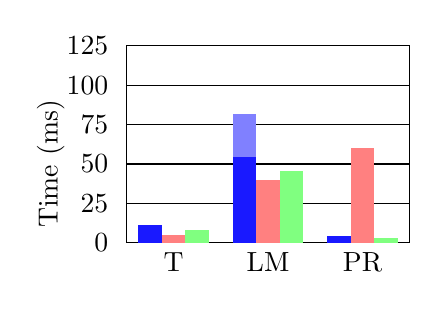
\begin{tikzpicture}
    \def\step{1.2}
    \draw (-\step*1.3,1) node[rotate=90]{Time~(ms)};
    \draw[xshift=-6mm] (0,0) grid[xstep=3*\step,ystep=25,xscale=1.,yscale=0.02] (3*\step, 125);
    \foreach \n/\x in {T/0,LM/\step, PR/2*\step} \draw (\x,0) node [below] {\n};
    \foreach \y in {0,25,...,125} \draw[yscale=0.02](-\step/1.7,\y)node[left]{\y};

    \draw[line width=3mm,color=blue!50,xshift=-3mm,xscale=1.,yscale=0.02] plot[ycomb] coordinates {(\step,81.5)};
    \draw[line width=3mm,color=blue!90,xshift=-3mm,xscale=1.,yscale=0.02] plot[ycomb] coordinates {(0,11.1) (\step,54.3) (2*\step,4.4)};
    \draw[line width=3mm,color=red!50,xshift=0mm,xscale=1.,yscale=0.02] plot[ycomb] coordinates {(0,4.6) (\step,39.8) (2*\step,60.0)};
    \draw[line width=3mm,color=green!50,xshift=3mm,xscale=1.,yscale=0.02] plot[ycomb] coordinates {(0,7.8) (\step,45.8) (2*\step,3.1)};
\end{tikzpicture}